\begin{surferPage}[Barth]{Het zesdegraadsoppervlak van Barth}
   Dit oppervlak van graad $6$ werd geconstrueerd door Wolf Barth in 1996.
    
    Het zesdegraadsoppervlak van Barth heeft in totaal $65$ singulariteiten.
%    (wenn man die $15$ im Bild nicht sichtbaren, ``unendlich fernen'', mitz�hlt)%
   Zoals kort na Barth's constructie door Jaffe en Ruberman werd aangetoond, is dit het maximale aantal singulariteiten op een zesdegraadsoppervlak --- dus Barth's wereldrecord kan niet meer verbeterd worden!


   Barth's constructie was een grote verrassing omdat men lang dacht dat een oppervlak van graad $6$ slechts $64$ singulariteiten kon hebben.

  Een opvallend kenmerk van de constructie is de icosahedrale symmetrie. De afbeelding hieronder toont een icosa\"eder en zijn symmetrievlakken:  
%    Die Abb.\ zeigt diesen platonischen K�rper und seine Symmetrie - Ebenen: 
%    und diese Ebenen gemeinsam mit der Barth Sextik in einem Bild.     
    % 
  \begin{center}
      \vspace*{-0.1cm}
      \begin{tabular}{@{}c@{\ \ }c@{\,}c@{}}
        \begin{tabular}{@{}c}
          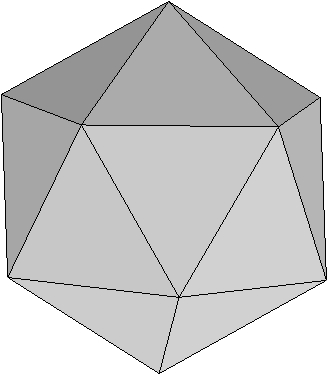
\includegraphics[width=1.4cm]{icosah}
        \end{tabular}
        &
        \begin{tabular}{@{}c}
          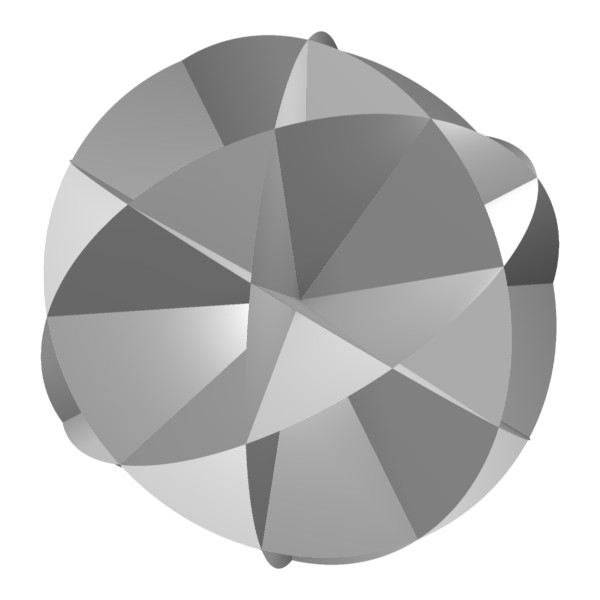
\includegraphics[width=1.4cm]{barth_sextic_planes}
        \end{tabular}
        &
        \begin{tabular}{c@{}}
          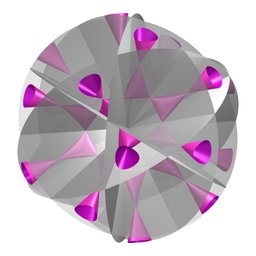
\includegraphics[width=1.4cm]{barth_sextic_and_planes}
        \end{tabular}
      \end{tabular}
    \end{center}
    \vspace*{-0.1cm}

    Dit zesdegraadsoppervlak voldoet aan de vergelijking 
    $P_6 - \alpha K^2=0,$ waar $P_6$
    slaat op de symmetrievlakken, $K=x^2+y^2+z^2-1$ het eenheidsboloppervlak is en $\alpha=\frac{1}{4}(2+\sqrt{5})$.
\end{surferPage}
